\section{Coresets and Sensitivity Sampling}

In this work, we are using the method of coresets
(see for example~\cite{munteanu-coresets-introduction})
to approach the problem of data reduction for the probit model.
The idea behind coresets is, that when given a
dataset $\mathcal{D}$, we are interested in selecting
only a small subset of observations
$\mathcal{C} \subseteq \mathcal{D}$, such that the objective
function evaluated on the (possible reweighted) subset $\mathcal{C}$
does not differ too much
from the objective function evaluated on the original dataset $\mathcal{D}$.

This approach will allow us to estimate the model parameters
efficiently on the ideally much smaller set $\mathcal{C}$,
when a full optimization on $\mathcal{D}$ could already
be infeasible for big datasets.
We are thus following the paradigm of \textit{sketch-and-solve},
i.e. first reducing the size of the original dataset and then solving
the optimization problem on the reduced dataset.

In order to work out a formal definition of when we call a subset
$\mathcal{C} \subseteq \mathcal{D}$ a coreset in the context of
probit regression, we first have to slightly extend the
concept of the model matrix, as we will need it for the coreset
definition.

\begin{definition}[Scaled model matrix]
    Let $\mathcal{D}=\{(x_i, y_i)\}_{i=1}^n$ be a $d$-dimensional dataset.
    Let $z_i = (2y_i - 1)x_i$ for all i in $[n]$.
    Then we call the matrix $Z \in \mathbb{R}^{n \times d}$, where the
    $i$-th row consists of the vector $z_i$ for all $i \in [n]$,
    the scaled model matrix of $\mathcal{D}$.
\end{definition}

This definition of the scaled model matrix is nothing particularly new,
it just formalizes the concept of factoring the labels into the
model matrix, which we already encountered when dealing with the
parameter estimation in section~\ref{sec:parameter-estimation}.

We are now ready for the coreset definition:

\begin{definition}[Coreset]
    \label{def:coreset}
    Let $\mathcal{D}=\{(x_i, y_i)\}_{i=1}^n$ be a $d$-dimensional dataset
    with scaled model matrix $Z \in \mathbb{R}^{n \times d}$ and
    a vector of positive sample weights $w \in \mathbb{R}_{>0}^n$.
    Let $\mathcal{C} \subseteq \mathcal{D}$ be a subset of $\mathcal{D}$
    of size $|\mathcal{C}| = k$
    with scaled model matrix $C \in \mathbb{R}^{k \times d}$ and
    a vector of positive sample weights $u \in \mathbb{R}_{>0}^k$.
    Let $\frac{1}{2} > \epsilon > 0$.
    We call $\mathcal{C}$ a $(1+\epsilon)$-coreset of $\mathcal{D}$
    for probit regression, if
    \begin{equation*}
        (1-\epsilon)f_Z^w(\beta) \leq f_C^u(\beta) \leq (1+\epsilon)f_Z^w(\beta)
        \quad \forall \beta \in \mathbb{R}^d,
    \end{equation*}
    where $f_Z^w(\beta) = \sum_{i=1}^n w_i g(z_i^T \beta)$ is the
    weighted objective function of the probit model.
\end{definition}

The size parameter $k = |\mathcal{C}|$ of a coreset usually depends
on the desired approximation quality $\epsilon$, as well as on
specific problem characteristics, such as the number of observations
$n$ as well as the dimensionality $d$ of the dataset.
When constructing coresets, we are interested in keeping this parameter
low in comparison to the total size of the dataset, i.e. we
usually require that at least $k \in O(\log{n})$, so that
the data reduction is actually meaningful.

In the next section, we will investigate if there are any
guarantees that can be given regarding the coreset size
without imposing any further restrictions on the dataset.
We will find out, that in the general case, it can't
be guaranteed that a reasonably small coreset always exists,
which rises the need for new restrictions on the datasets
under study.

\subsection{Lower Bounds for Coreset Size in the General Case}

\begin{theorem}
    There exists a $d$-dimensional dataset $\mathcal{D}$ of size
    $|\mathcal{D}| = n$, such
    that any $(1+\epsilon)$-coreset $\mathcal{C}$ of $\mathcal{D}$
    for probit regression has a size $k = |\mathcal{C}|$
    of at least $k \in \Omega\left(\frac{n}{\log{n}}\right)$.
\end{theorem}
\begin{proof}
    We can construct such a  dataset by showing
    how coresets can be used in a
    communication protocol for the so called INDEX communication game
    to encode a message.
    Since there exists a lower bound on the minimum
    message length of the INDEX game (see~\cite{index}),
    we can use it to derive a lower bound on the
    coreset size.
    The same technique was also used in~\cite{on-coresets} to find
    lower bounds for coresets of logistic regression and is here slightly
    adapted for probit regression.

    The INDEX game consists of two players, Alice and Bob.
    Alice is given a random binary string $m \in \{0, 1\}^n$ of $n$ bits
    and Bob is given an index $i \in [n]$.
    The goal is for Alice to send a message to Bob that allows
    Bob to obtain the value $m_i$ of Alice's binary string $m$.
    It was shown in~\cite{index}, that the minimum length of a message
    sent by Alice that still allows Bob to obtain $m_i$ with
    constant probability is in $\Omega(n)$ bits.
    We will now see how a coreset for probit regression can be used
    to encode such a message.

    The first step is for Alice to convert her binary string $m$ into
    a two-dimensional dataset $\mathcal{D}$ as follows:
    For each entry $m_j$ of her binary string where $m_j = 1$, she adds
    a point
    \begin{equation*}
        x_j = \left( \cos{\left(2 \pi \frac{j}{n}\right)},
        \sin{\left(2 \pi \frac{j}{n}\right)} \right)^T
    \end{equation*}
    to her set $\mathcal{D}$ and labels it with $y_j = 1$,
    ending up with the dataset
    \begin{equation*}
        \mathcal{D} = \{(x_j, 1)\}_{j \in \{i \in [n]:\ m_i = 1 \}}.
    \end{equation*}
    As we can see, all of these points are on the unit circle and all
    of them are labeled with $1$.

    The next step for her is to construct a
    $(1+\epsilon)$-coreset $\mathcal{C}$ of $\mathcal{D}$
    for probit regression with sample weights $u \in \mathbb{R}^k_{>0}$
    and to transmit both the coreset and the weight vector to Bob.
    We will later see, how
    large the size $|\mathcal{C}|=k$ of this coreset must be,
    so that Bob can still
    obtain the value of $m_i$ with constant probability.

    As soon as Alice's coreset $\mathcal{C}$ arrives at Bob,
    Bob can use it to obtain the value of $m_i$.
    To do this, Bob first adds two new points
    \begin{equation*}
        q_1 = \left( \cos{\left(2 \pi \frac{i - 0.5}{n}\right)},
        \sin{\left(2 \pi \frac{i - 0.5}{n}\right)} \right)^T
    \end{equation*}
    and
    \begin{equation*}
        q_2 = \left( \cos{\left(2 \pi \frac{i + 0.5}{n}\right)},
        \sin{\left(2 \pi \frac{i + 0.5}{n}\right)} \right)^T
    \end{equation*}
    to the set and labels both points with $0$ (see figure~\ref{fig:index}),
    i.e. Bob now has the dataset
    \begin{equation*}
        \mathcal{C}' = \mathcal{C} \cup \{(q_1, 0)\} \cup \{(q_2, 0)\}.
    \end{equation*}

    Next, he uses this new dataset $\mathcal{C}'$ with
    scaled model matrix $C'$ to
    minimize the weighted objective function
    $f_{C'}^u$ of the probit model,
    by using the Newton-Raphson optimization algorithm.

    Taking a look at figure~\ref{fig:index}, it becomes evident,
    that Bobs points $q_1$ and $q_2$ are linearly separable from
    the other points if and only if Alice didn't add a point
    $x_i$, i.e. if $m_i = 0$.
    He can use the results of the optimization procedure to
    make a distinction between the two cases
    (which then allows him to determine the value of $m_i$)
    like this:

    In the case of $m_i=1$, Bobs points are not linearly separable from
    Alices points, which means that there must occur at least one
    misclassification at a cost of $g(0) = \log(2)$.
    Because Bobs dataset $\mathcal{C}'$ allows him to obtain a
    $(1 \pm \epsilon)$-approximation of the cost function, he can
    check if the Newton-Raphson algorithm converges to
    a cost of at least $(1 - \epsilon) \log(2) \geq \frac{1}{2} \log(2)$.
    In this case, he knows that Alice must have added the point $x_i$,
    which means that $m_i=1$.

    Conversely, if at any point during the optimization procedure
    the cost function drops below
    $\frac{1}{2} \log(2)$
    and approaches zero, Bob knows that Alice didn't add the point
    $x_i$, because his dataset $\mathcal{C}'$ is linearly separable.
    This will allow him to conclude that $m_i = 0$.

    There is one special case that has to be dealt with in order for this
    protocol to work. If Alice's coreset $\mathcal{C}$
    only consists of the single point
    $x_i$, Bob's points $q_1$ and $q_2$ could still be linearly seperated
    although Alice added $x_i$.
    The workaround to this is simple though:
    Bob can always just add two more
    points at the locations of $x_{i-1}$ and $x_{i+1}$ and label them with 1.
    Now, $q_1$ and $q_2$ can only be linearly seperated from the
    other points if and only if Alice didn't add a point $x_i$.

    Let us now see how big the size $k$ of Alice's coreset must be
    for this protocol to work with constant probability.
    In~\cite{index} it was shown, that the minimum length of a message
    that Alice must send in order for the protocol to work
    is in $\Omega(n)$ bits.
    Since each of the points that Alice created can be encoded in
    $\log(n)$ space, it follows from the lower bound that
    $\Omega(n) \subseteq \Omega(k \log(n))$, so $k$ must be in
    $\Omega\left(\frac{n}{\log(n)}\right)$.

    We can conclude, that if there existed a $(1 + \epsilon)$-coreset
    of $\mathcal{D}$
    for probit regression with size $k \in o\left(\frac{n}{\log(n)}\right)$,
    it would contradict the minimum message length of
    the INDEX communication game, which proves the theorem.
\end{proof}

\begin{figure}
    \centering
    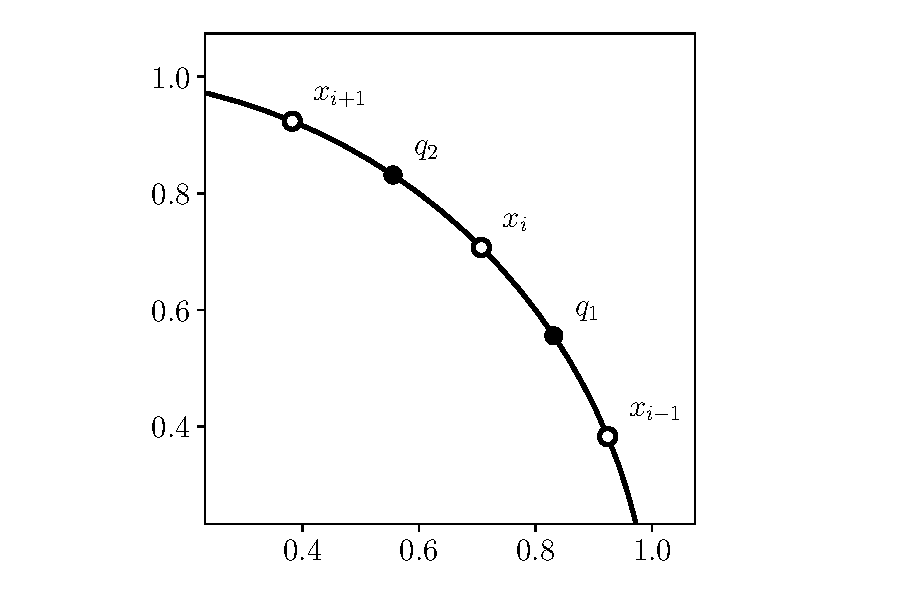
\includegraphics[width=0.8\textwidth]{figures/index.pdf}
    \caption{Bob places two points $q_1$ and $q_2$ in such a way
        on the unit circle, that they can be linearly seperated from the other
        points if and only if Alice didn't place a point at $x_i$.}
    \label{fig:index}
\end{figure}

\subsection{Sensitivity Sampling}

\subsubsection{Theoretical Foundations}

\begin{definition}[\cite{langberg-schulman-sensitivities}]
    \label{def:sensitivity}
    Let $F = \{ g_1, ..., g_n \}$ be a set of functions,
    $g_i: \mathbb{R} \rightarrow \mathbb{R}_{\geq 0}, \ i=1,...,n$ weighted by
    $w \in \mathbb{R}^n_{>0}$.
    The sensitivity of $g_i$ for $f_w(\beta) = \sum_{i=1}^n w_i g_i(\beta)$ is defined as
    \begin{equation*}
        \varsigma_i = \sup_{\beta \in \mathbb{R}^d, \ f_w(\beta) > 0} \frac{w_i g_i(\beta)}{f_w(\beta)}.
    \end{equation*}
    The total sensitivity, i.e. the sum of the sensitivities is $\mathfrak{S} = \sum_{i=1}^n \varsigma_i$.
\end{definition}

\begin{definition}[\cite{feldman-langberg-coresets}]
    A range space is a pair $\mathfrak{R} = (F, \mathcal{R})$, where F is a set
    and $\mathcal{R}$ is a family (set) of subsets of F, called
    ranges.
\end{definition}

\begin{definition}[\cite{feldman-langberg-coresets}]
    The VC-dimension $\Delta(\mathfrak{R})$ of a range space $\mathfrak{R} = (F, \mathcal{R})$ is
    the size $|G|$ of the largest subset $G \subseteq F$ such that
    \begin{equation*}
        \left| \left\{ G \cap \textup{range} \ | \ \textup{range} \in \mathcal{R} \right\} \right|
        = 2^{|G|},
    \end{equation*}
    i.e. $G$ is shattered by $\mathcal{R}$.
\end{definition}

\begin{definition}[\cite{feldman-langberg-coresets}]
    Let $F$ be a finite set of functions mapping from $\mathbb{R}^d$ to $\mathbb{R}^{\geq 0}$.
    For every $\beta \in \mathbb{R}^d$ and $r \geq 0$, let
    \begin{equation*}
        \textup{range}(F, \beta, r) = \left\{ f \in F \ | \  f(\beta) \geq r  \right\}
    \end{equation*}
    and let
    \begin{equation*}
        \mathcal{R}(F) = \left\{ \textup{range}(F, \beta, r) \ | \ \beta \in \mathbb{R}^d, \ r \geq 0  \right\}.
    \end{equation*}
    Then we call $\mathfrak{R}_F := (F, \mathcal{R}(F))$ the range space induced by F.
\end{definition}

\begin{theorem}[\cite{braverman-feldman-coresets, big-data-tiny-data}]
    Let $\mathcal{F} = \{ f_1, ..., f_n \}$ be a set of functions,
    $f_i: \mathbb{R} \rightarrow \mathbb{R}^{\geq 0}, \ i=1,...,n$ weighted by
    $w \in \mathbb{R}^n_{>0}$.
    Let $\epsilon, \delta \in (0, \frac{1}{2})$.
    Let $s_i \geq \varsigma_i$.
    Let $S = \sum_{i=1}^n s_i \geq \mathfrak{S}$.
    Given $s_i$, one can compute in time $O(|\mathcal{F}|)$ a set
    $\mathcal{R} \subseteq \mathcal{F}$ of
    \begin{equation*}
        O \left( \frac{S}{\epsilon^2} \left( \Delta \log S + \log \left( \frac{1}{\delta} \right) \right) \right)
    \end{equation*}
    weighted functions such that with probability $1 - \delta$ we have
    for all $\beta \in \mathbb{R}^d$ simultaneously
    \begin{equation*}
        \left| \sum_{f \in \mathcal{F}} w_i f_i(\beta) - \sum_{f \in \mathcal{R}} u_i f_i(\beta) \right| \leq \epsilon \sum_{f \in \mathcal{F}} w_i f_i(\beta)
    \end{equation*}
    where each element of $\mathcal{R}$ is sampled independently with probability
    $p_j = \frac{s_j}{S}$ from $\mathcal{F}$, $u_i = \frac{S w_j}{s_j |\mathcal{R}|}$
    denotes the weight of a function $f_i \in \mathcal{R}$ that corresponds to
    $f_j \in \mathcal{F}$, and where $\Delta$ is an upper bound on the
    VC-dimension of the range space $\mathfrak{R}_{\mathcal{F}^*}$ induced by
    $\mathcal{F}^*$. $\mathcal{F}^*$ is the set of functions $f_j \in \mathcal{F}$
    scaled by $\frac{S w_j}{s_j |\mathcal{R}|}$.
\end{theorem}

\subsubsection{Constructing the Coreset}
